\documentclass[a4paper]{report}

\usepackage[utf8]{inputenc}
\usepackage[portuges]{babel}
\usepackage{graphicx}
\usepackage{a4wide}
\usepackage[pdftex]{hyperref}
\usepackage{float}
\usepackage{graphicx}
\usepackage{indentfirst}

\title{Projeto de Laboratórios de Informática III\\Grupo 1}
\author{Catarina Machado (a81047) \and Cecília Soares (a34900) \and João Vilaça (a82339)}
\date{\today}


\begin{document}

\maketitle

\begin{abstract}
O presente relatório descreve o projeto realizado no âmbito da disciplina de
\emph {Laboratórios de Informática III} (LI3), ao longo do segundo semestre,
do segundo ano, do Mestrado Integrado em Engenharia Informática da Universidade
do Minho.

O objetivo do projeto foi desenvolver um sistema capaz de processar a informação
contida em ficheiros XML para responder a um conjunto de interrogações de forma
eficiente, utilizando, para isso, a linguagem de programação C. Neste documento
descrevemos sucintamente as decisões de implementação e as limitações da solução
adoptada.

\end{abstract}

\tableofcontents

\chapter{Introdução}
\label{ch:intro}

O presente relatório foi elaborado no âmbito da unidade curricular \emph {Laboratórios
de Informática 3} (LI3), ao longo do segundo semestre, do segundo ano, do Mestrado
Integrado em Engenharia Informática da Universidade do Minho, e tem como objetivo
descrever as tarefas desenvolvidas para criar um sistema capaz de processar as
informações contidas em ficheiros XML para responder a um conjunto de
interrogações de forma eficiente, utilizando a linguagem de programação C.


\section{Descrição do Problema}
\label{sec:problema}

O nosso trabalho visou implementar um sistema capaz de recolher e tratar dados
armazenados em ficheiros XML, usando, para tal, a linguagem de programação
imperativa C.

Os ficheiros em formato XML que deveriam ser processados continham informação referente ao
website \textit{Stack Overflow}. Este site foi criado em 2008 por Jeff Atwood e Joel
Spolsky para que programadores e entusiastas possam expor as suas dúvidas e
dificuldades na área, funcionando como um fórum em que os usuários fazem
perguntas e respondem a dúvidas dos seus pares. Além disso, podem ainda votar
em questões e repostas que considerem pertinentes, obtendo pontos de reputação
e medalhas pela qualidade da sua intervenção.

Em concreto, o trabalho prendia-se em extrair a informação necessária dos vários
ficheiros, de forma a conseguirmos responder a 11 interrogações relacionadas com
o conteúdo dos ficheiros da forma mais eficiente possível, isto é, tendo especial
atenção ao tempo de execução do programa, bem como ao encapsulamento dos dados.

Por último, listamos as onze interrogações predefinidas.
\begin{itemize}

\begin{item} Dado o identificador de um post, a função deve retornar
o título do post e o nome do autor. Se o post for uma resposta, a função deverá
retornar as informações da pergunta correspondente;\end{item}
\begin{item} Pretende obter o top N utilizadores com maior número
de posts de sempre. Para isto, devem ser considerados tanto perguntas
quanto respostas dadas pelo respectivo utilizador;\end{item}
\begin{item} Dado um intervalo de tempo arbitrário, obter o número
total de posts (identificando perguntas e respostas separadamente) neste
período;\end{item}
\begin{item} Dado um intervalo de tempo arbitrário, retornar todas
as perguntas contendo uma determinada tag. O retorno da função deverá ser
uma lista com os IDs das perguntas ordenadas em cronologia inversa\end{item}
\begin{item} Dado um ID de utilizador, devolver a informação do
seu perfil (short bio) e os IDs dos seus 10 últimos posts (perguntas ou respostas),
ordenados por cronologia inversa;\end{item}
\begin{item} Dado um intervalo de tempo arbitrário, devolver os IDs das N
respostas com mais votos, em ordem decrescente do número de votos; O número de
votos deverá ser obtido pela diferença entre Up Votes e Down Votes.\end{item}
\begin{item} Dado um intervalo de tempo arbitrário, devolver as IDs das N
perguntas com mais respostas, em ordem decrescente do número de respostas.\end{item}
\begin{item} Dado uma palavra, devolver uma lista com os IDs de N perguntas cujos
títulos a contenham, ordenados por cronologia inversa;\end{item}
\begin{item} Dados os IDs de dois utilizadores, devolver as últimas N perguntas
(cronologia inversa) em que participaram dois utilizadores específicos.\end{item}
\begin{item} Dado o ID de uma pergunta, obter a melhor resposta.
Para isso, deverá usar a função:
(Score x 0.45) + (Reputacao x 0.25) + (Votos x 0.2) + (Comtentarios x 0.1)\end{item}
\begin{item} Dado um intervalo arbitrário de tempo, devolver os identificadores
das N tags mais usadas pelos N utilizadores com melhor reputação.
Em ordem decrescente do número de vezes em que a tag foi usada.\end{item}

\end{itemize}

\section{Ficheiros XML}
\label{sec:xml}

De todos os ficheiros XML colocados à nossa disposição (Votes, Tags, Users,
PostLinks, Posts, PostHistory, Comments e Badges) e que se destinavam a dar resposta
às supra referidas interrogações decidimos que apenas iriamos precisar de carregar
algumas informações contidas em três dos oito ficheiros mencionados.
Os ficheiros selecionados para efetuar o \textit{parser} da informação relevante
foram, Tags.xml, Users.xml e Posts.xml. \par
No ficheiro Tags.xml retiramos somente o identificar da tag (id) e o nome da mesma
(TagName). \par
No que concerne ao ficheiro Users.xml, recolhemos a informação relativa ao identificador
do utilizador (id), à sua reputação (Reputation), ao seu nome (DisplayName) e ao seu
perfil (AboutMe). \par
Por último, quanto ao ficheiro Posts.xml fizemos o \textit{parser} do identificador
do post (id); do tipo de post (PostTypeId); do utilizador que publicou o post
(OwnerUserId); do seu título (Title); das suas tags (Tags); da pontuação obtida
(Score); do número de comentários que foram feitos (CommentCount); do número de
favoritos (FavoriteCount); no caso de ser uma resposta, do número da pergunta a
que se refere essa resposta (ParentId) e, finalmente, da sua data de criação
(CreationDate).

\section{Concepção da Solução}
\label{sec:solucao}

Para resolvermos este problema foram cruciais três momentos. Numa primeira fase,
definimos a estrutura de dados que consideramos que melhor solucionaria o nosso
problema. Posteriormente, analisamos as vantagens e desvantagens das diferentes
alternativas para fazer a leitura dos dados e a recolha da informação relevante.
A nossa opção recaiu na utilização da API SAX para fazer o \textit{parser} da
informação, dado que permite o acesso serial ao conteúdo de um documento XML de
forma orientada a eventos, aquilo a que chamam \textit{event-based parser} para
os documentos XML.
Finalmente, na última etapa do projeto concentramo-nos em responder
às diferentes \textit{queries}.

O código subjacente à solução proposta pode ser encontrado no repositório:

\begin{center}
\emph{https://github.com/dium-li3/Grupo1}.
\end{center}

O restante deste relatório está organizado da seguinte forma: o
Capítulo~\ref{ch:estruturadedados} descreve as estruturas de dados adoptadas,
ao passo que o Capítulo~\ref{ch:implementacao}  apresenta e discute a solução
proposta para a resolução do problema. O relatório termina com conclusões no
Capítulo~\ref{ch:conclusao}, onde é também apresentada uma análise crítica dos
resultados obtidos.



\chapter{Estrutura de Dados}
\label{ch:estruturadedados}

Para desenvolvermos este trabalho adotamos as seguintes estruturas de dados:

\begin{verbatim}

typedef struct TCD_community {
  GHashTable * users;
  GHashTable * questions;
  GHashTable * answers;
  GPtrArray * tmp_questions;
  GList * questionsList;
  GPtrArray * day;
  GHashTable * tags;
} TCD_community;

\end{verbatim}

Explicar porquê optamos pelas hashtables e porquê optamos pelas demais Estruturas
de dados e não optamos por outras??????
Explicar porque há 3 diferentes formas de aceder a questions.
Dizer quais são os elementos de cada estrutura.

\begin{verbatim}

typedef struct users {
  long user_id;
  char * shortbio;
  char * username;
  int reputation;
  int n_posts;
  GArray * last_posts;
} users;

\end{verbatim}

A estrutura de dados users contém o id do utilizador, o seu perfil, o seu nome,
a sua reputação, o número total de posts desse utilizador (i.e. perguntas e respostas),
bem como um GArray contendo todos os posts do utilizador (perguntas e respostas) no
formato \textit{postAndDate}.
Esta estrutura encerra informações necessárias para responder às interrogações 1,
5, 8 e 10.

\begin{verbatim}

typedef struct questions {
  long post_id;
  postDate pd;
  long user_id;
  char * title;
  char * tags;
  int n_answer_votes;
  int n_answers;
  GPtrArray * answers;
} questions;

\end{verbatim}

A estrutura de dados questions contém o id da pergunta, a sua data no formato
\textit{postAndDate}, o id do utilizador que publicou a pergunta, o seu título,
as suas tags, o número total de votos das suas respostas, o número total de
respostas que obteve, bem como um GPtrArray com todas as respostas de cada
pergunta no formato formato \textit{answers}.
Esta estrutura encerra informações necessárias para responder às interrogações 1,
4, 7, 8 e 11.


\begin{verbatim}

typedef struct answers {
  long user_id;
  long answer_id;
  long parent_id;
  int score;
  int up_votes; //retirar
  int down_votes; // retirar
  int comment_count;
} answers;

\end{verbatim}

A estrutura de dados answers contém o id do utilizador, o id da resposta, o id da
pergunta a que essa resposta se refere, a sua pontuação e os seus comentários.
Esta estrutura encerra informações necessárias para responder às interrogações 1,
6, 9 e 10.

\begin{verbatim}

typedef struct day {
  int day;
  int month;
  int year;
  int n_questions;
  int n_answers;
  GPtrArray * questions;
  GPtrArray * answers;
} day;

\end{verbatim}



\begin{verbatim}

typedef struct postAndDate {
    long post_id;
    int year, month, day, hour, min, sec, mili;
} postAndDate;

\end{verbatim}


\begin{verbatim}

typedef struct tags {
  int id;
  char * nameTag;
  int value;
} tags;

\end{verbatim}




\chapter{Implementação}
\label{ch:implementacao}

\section{Organização Geral}
\label{sec:organizacao}

O trabalho é composto por vários módulos, tendo sido os que a seguir se descrevem
criados por nós, consoante as necessidades que fomos detectando.

\begin{itemize}
\begin{item} main.c - main do programa\end{item}
\begin{item} 00load.c - contem as funções necessárias para recolher e carregar os
dados necessários dos ficheiros XML.\end{item}
\begin{item} answers.c - todas as funções necessárias para aceder à estrutura de
dados answers\end{item}
\begin{item} day.c - todas as funções necessárias para aceder à estrutura de
dados day\end{item}
\begin{item} questions.c - todas as funções necessárias para aceder à estrutura de
dados questions\end{item}
\begin{item} struct.c - todas as funções necessárias para inicializar e aceder à
estrutura de dados TCD\_community\end{item}
\begin{item} tags.c - todas as funções necessárias para aceder à estrutura de
dados tags\end{item}
\begin{item} users.c - todas as funções necessárias para aceder à estrutura de
dados users\end{item}
\begin{item} postDate.c - todas as funções necessárias para aceder à estrutura de
dados postDate\end{item}
\begin{item} 01TitleUserName.c - responde à interrogação n.º 1.\end{item}
\begin{item} 02TopMostActive.c - responde à interrogação n.º 2.\end{item}
\begin{item} 03totalPostDate.c - responde à interrogação n.º 3.\end{item}
\begin{item} 04questionsWithTag.c - responde à interrogação n.º 4.\end{item}
\begin{item} 05UserInfo.c - responde à interrogação n.º 5.\end{item}
\begin{item} 06mostVotedAnswers.c - responde à interrogação n.º 6.\end{item}
\begin{item} 07mostAnsweredQuestions.c - responde à interrogação n.º 7.\end{item}
\begin{item} 08titlesWithWord.c - responde à interrogação n.º 8.\end{item}
\begin{item} 09bothParticipated.c - responde à interrogação n.º 9.\end{item}
\begin{item} 10BetterAnswer.c - responde à interrogação n.º 10.\end{item}
\begin{item} 11mostUsedBestRep.c - responde à interrogação n.º 11.\end{item}
\begin{item} 12clean.c - liberta o espaço de memória que não está sendo utilizado.\end{item}
\end{itemize}


O encapsulamento de todos os dados foi garantido por \textbf{\textit{forward declaration}}
de todas as estruturas de dados, sendo os seus atributos somente acessíveis através
de funções ``getters e setters''. De facto, os ficheiros headers criados impossibilitam
que os atributos das diversas estruturas de dados criadas sejam acedidos diretamente.
Por exemplo, a estrutura de dados que contém todos as informações relevantes e
referentes ao usuário foi definida no ficheiro users.c da seguinte forma:

\begin{verbatim}

typedef struct users {
  long user_id;
  char * shortbio;
  char * username;
  int reputation;
  int n_posts;
  GArray * last_posts;
} users;

\end{verbatim}

sendo que o acesso aos elementos de users só é possível através das funções
``getters e setters'', como por exemplo, \textit{getUserId} ou
\textit{setUserId}, já que o ficheiro header users.h possui apenas a declaração
\textit{typedef struct users * Users}.

\section{Leitura e Recolha de Dados}

A primeira fase do nosso projeto passou por determinar e criar a estrutura de dados
que melhor se adequava ao problema em questão.
Numa segunda fase, estudamos qual a melhor forma de ler e recolher os dados armazenados
nos ficheiros XML e, pesadas todas as vantagens e desvantagens, optamos por fazer o
\textit{parser} dos dados com recurso ao SAX \textit{(Simple API for XML)},
em detrimento do DOM \textit{(Document Object Model)}. \par
O DOM é um modelo que representa documentos XML numa estrutura
em forma de árvore, designada de árvore DOM. Apesar do mesmo ser mais simples de utilizar,
tornava o programa substancialmente mais lento, visto que consumia mais memória porque os ficheiros
XML a serem processados eram grandes, resultando na construção de uma árvore DOM com toda a informação
contida nos mesmos, a qual permanecia na memória enquanto estivesse a ser utilizada. Acresce que
as diversas funcionalidades que o DOM possui, tais como, navegar pelos nós, remover, editar e apagar
os nós da árvore DOM, acabam por gerar uma sobrecarga da memória sendo, concomitantemente,
desnecessárias para a realização do projeto. \par
Por seu turno, a SAX efectua o \textit{parser} de ficheiros em formato XML, definindo
funções que são executadas quando determinado evento ocorre - ``callbacks''. O consumo de memória
é reduzido, comparativamente com o DOM, uma vez que a memória utilizada corresponde somente às
informações que estão sendo processadas pelas ``callbacks''. \par

A leitura e recolha dos dados contidos nos ficheiros XML estão implementadas no
ficheiro 00load.c, o qual foi construído com tendo por base o código encontrado em:
\begin{center}
\emph{https://gist.github.com/cooldaemon/106870}.
\end{center}

Existem 4 ``callbacks'', isto é, todas as funções cujos nomes são
iniciados por OnStartElement, as quais carregam toda a informação que consideramos
relevante para as diversas estruturas de dados que definimos. \par
Esse processo é feito da seguinte forma: a função main chama a função load que,
por sua vez, chama a função read\_xmlfile, descrita de seguida:

\begin{verbatim}

static int read_xmlfile(FILE *file, char *dump_file_name) {
  char chars[1024];
  int result = fread(chars, 1, 4, file);
  if (result <= 0) {
      return 1;
  }
  xmlSAXHandler SAXHander = make_sax_handler(dump_file_name);

  xmlParserCtxtPtr ctxt = xmlCreatePushParserCtxt(&SAXHander, NULL,
                                                  chars, result, NULL);

  while ((result = fread(chars, 1, sizeof(chars), file)) > 0) {
      if(xmlParseChunk(ctxt, chars, result, 0)) {
         xmlParserError(ctxt, "xmlParseChunk");
         return 1;
      }
  }
  xmlParseChunk(ctxt, chars, 0, 1);

  xmlFreeParserCtxt(ctxt);
  xmlCleanupParser();
  return 0;
}
\end{verbatim}

A função read\_xmlfile começa por verificar o \textit{encoding}
ao ler 4 bytes para um \textit{buffer}. De seguida, executa a função make\_sax\_handler,
que define quais as ``callbacks'' a serem utilizadas pelo programa. Posteriormente, inicializa
o SAX e vai lendo o conteúdo do ficheiro XML respectivo, passando a informação
relevante para o \textit{buffer} e, posteriormente, faz \textit{parser} desse \textit{buffer}.
Note-se que quando esta função estiver a executar o \textit{parser} dos dados, através da
função xmlParseChunk chama as diversas ``callbacks'' sempre que se justifique.

As ``callbacks'' são funções que recebem três parâmetros:

\begin{itemize}

\begin{item}void *ctx - um apontador para uma estrutura de dados do Sax \end{item}

\begin{item}const xmlChar *element\_name - um apontador para o nome de um elemento XML\end{item}

\begin{item}const xmlChar **attributes - um apontador para um array com os atributos do elemento\end{item}

\end{itemize}

Convém esclarecer que nos ficheiros xml, um elemento é constituído por uma tag-inicial,
um conteúdo e uma tag-final. Um elemento pode conter outra informação em atributos (meta-informação),
cujos valores devem ser colocados entre aspas, como por exemplo,
\begin{verbatim}
<row Id="3" TagName="sms" Count="897" ExcerptPostId="13195" WikiPostId="13194"/>
\end{verbatim}

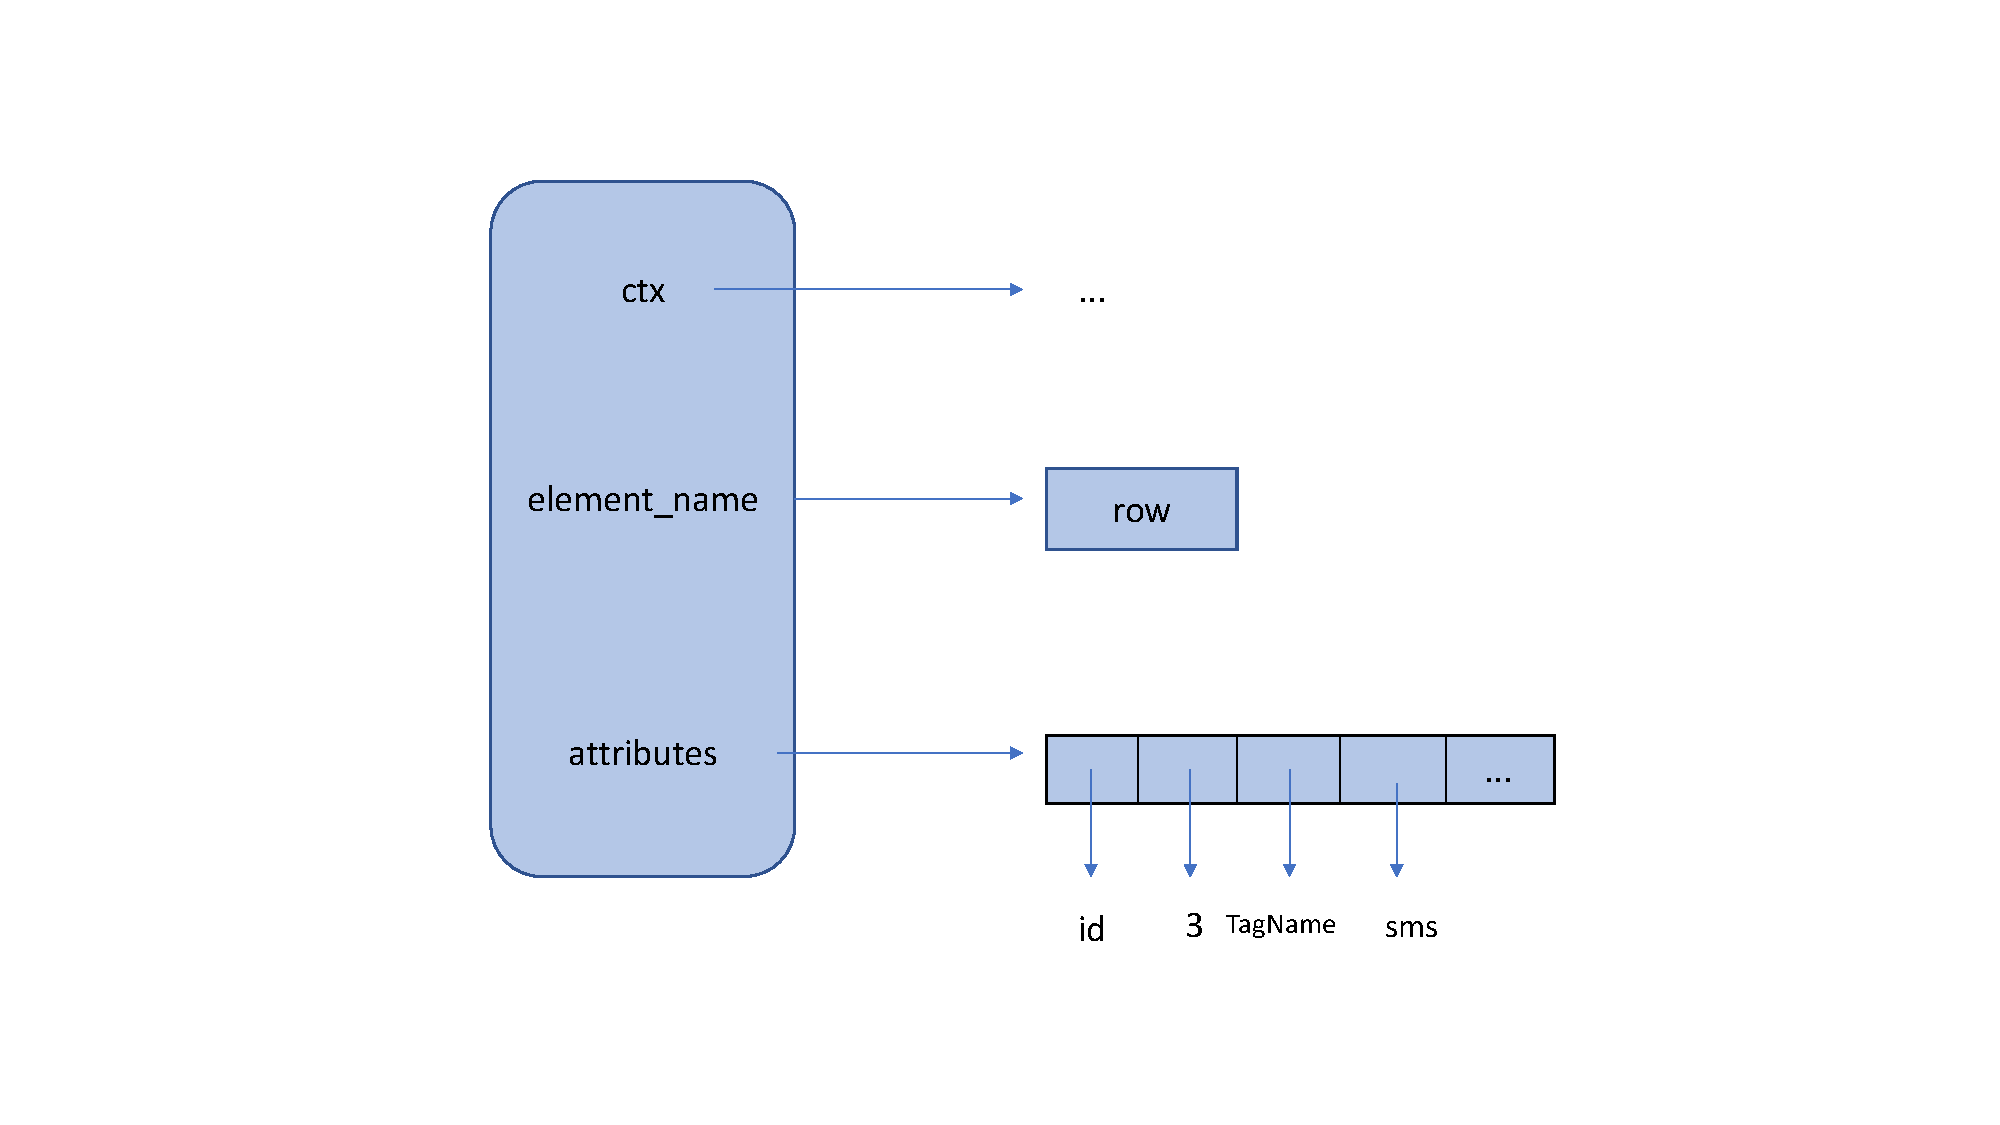
\includegraphics[scale=0.4]{xmlelements.pdf}

É através destas funções que conseguimos extrair o conteúdo dos elementos, bem como dos
atributos que consideramos relevante dos diversos ficheiros XML e carregamos as informações
para as estruturas de dados adequadas.

Finalmente, a última etapa do nosso projeto prendeu-se com a resposta às diversas
\textit{queries}, as quais passamos a explicar no próximo capítulo.

\section{Queries}
\label{sec:queries}

\subsection*{Query 1}
\label{sec:query1}

\textbf{“Dado o identificador de um post, a função deve retornar
um par com o título do post e o nome (não o ID) de utilizador do autor. Se o post
for uma resposta, a função deverá retornar informações (título e utilizador)
da pergunta correspondente.”}


Na resposta a esta query, começamos por verificar se o id do post passado como
parâmetro  para a função identifica uma pergunta. No caso da resposta ser negativa
verificamos se esse id identifica alguma resposta contida na GHashTable answers. \par
Na hipótese de ser uma pergunta, com o auxílio da estrutura de dados questions
conseguimos obter o título do post e o id do utilizador, através do qual, procurando
na GHashTable users conseguimos saber se o usuário existe e, caso exista, obter
todas as suas informações relevantes e, posteriormente, extrair o seu nome através
da função getUsername que devolve um username. Desta forma, conseguimos devolver o par
pretendido, o título do post e o nome do utilizador. \par
No caso do id passado como parâmetro para a função identificar uma resposta, determinamos
a que pergunta esta se refere e procuramos na GHashTable questions essa pergunta
para, de seguida, seguirmos o procedimento descrito no parágrafo anterior.

\subsection*{Query 2}
\label{sec:query2}

\textbf{“Função que devolve o top N utilizadores com maior número
de posts de sempre. Para isto, são considerados tanto perguntas
quanto respostas dadas pelo respectivo utilizador.”}

\begin{verbatim}

typedef struct totalPosts {
  long user_id;
  int n_posts;
} totalPosts;

\end{verbatim}

A estrutura de dados totalPosts é composta por um long que identifica o utilizador
e um inteiro que traduz o número de posts daquele mesmo utilizador.
Esta estrutura foi criada especificamente para responder à interrogação 2.

Para respondermos a esta interrogação começamos por criar a estrutura de dados
totalPosts, que, tal como referimos anteriormente, encerra o id do usuário e o número
de posts que publicou. Estas informações vão constar de cada posição de uma garray
entretanto criado e que irá ser preenchido com a informação resultante de percorrer
toda a GHashTable users. De seguida ordenamos o referido garray, o qual passará a
conter todos os users, bem como o total de post que cada um publicou, por ordem
decrescente do número de posts. Por último, com o auxílio de um ciclo com N iterações,
inserirmos os N utilizadores com mais posts de sempre na lista que é devolvida por
esta função.

\subsection*{Query 3}
\label{sec:query3}

\textbf{“Dado um intervalo de tempo arbitrário,
obter o número total de posts (identificando perguntas e respostas separadamente) neste período.”}

Uma vez que na nossa estrutura Day já temos uma variável que nos diz o número total de perguntas
e o número total de respostas efetuadas num determinado dia, para sabermos o
número total de cada uma delas durante um intervalo de tempo criámos duas novas
variáveis na nossa função da query 3: \textsf{'n\_questions'} e \textsf{'n\_answers'},
e incrementámo-las com o valor das perguntas e respostas efetuadas, respetivamente,
durante os dias passados como parâmetro.

No final de percorridos todos os dias, adicionamos as duas variáveis da nossa função a um LONG\_pair, e retornamo-lo.


\subsection*{Query 4}
\label{sec:query4}

\textbf{“Dado um intervalo de tempo arbitrário, retornar todas as perguntas contendo uma determinada tag.
O retorno da função deverá ser uma lista com os IDs das perguntas ordenadas em cronologia inversa."}

Para esta query, tirando partido da nossa estrutura Day, que tem um GPtrArray com
os apontadores das perguntas do dia em questão, começamos por percorrer cada pergunta desse array
da última data passada como parâmetro e comparamos as suas tags com a tag passada como argumento.
Deste modo, se a pergunta tiver a tag desejada inserimos o seu ID numa LONG\_list.
Vamos percorrendo os dias da “Date end” para a “Date begin”.

No final de consultarmos todas as perguntas do intervalo de tempo temos a LONG\_list preenchida.
Esta LONG\_list tem os IDs das perguntas ordenadas por cronologia inversa uma vez que
vamos preenchendo a lista do dia mais recente para o dia mais antigo.



\subsection*{Query 5}
\label{sec:query5}

\subsection*{Query 6}
\label{sec:query6}

\textbf{“Dado um intervalo de tempo arbitrário, devolver os IDs das N respostas
com mais votos, em ordem decrescente do número de votos; O número de votos deverá
ser obtido pela diferença entre Up Votes (UpMod6) e Down Votes (DownMod)."}

Nesta query utilizamos um GPtrArray auxiliar. Ao percorrer os dias do intervalo
de tempo fornecido como parâmetro inserimos no array auxiliar os apontadores das
respostas que iam aparecendo.

Depois de percorrer todos os dias temos um array auxiliar com todas as respostas
efetuadas nesse intervalo de tempo. Consequentemente, ordenamos o array pelo número
de votos (no inicio do array está a resposta com mais votos e no fim a resposta com menos votos).

Para sabermos as N respostas com mais votos, consultamos o nosso array auxiliar
e retiramos dele o ID das primeiras N respostas que aparecem.

Assim, temos a LONG\_list pedida, por ordem decrescente do número de votos.



\subsection*{Query 7}
\label{sec:query7}

\textbf{“Dado um intervalo de tempo arbitrário, devolver as IDs das N perguntas
com mais respostas, em ordem decrescente do número de respostas."}

Para a resolução desta query também recorremos a um array auxiliar, porém
desta vez com apontadores para perguntas.

Utilizamos o mesmo raciocínio da Query 6, mas agora fomos percorrendo o intervalo
de tempo e adicionando ao nosso array auxiliar os apontadores para as perguntas.
No fim do array preenchido, ordenamo-lo segundo o critério de maior número de respostas.

Retiramos os primeiros N elementos do array e devolvemos os determinados IDs
numa LONG\_list, que se encontra então ordenada decrescentemente segundo o número de respostas.


\subsection*{Query 8}
\label{sec:query8}

\subsection*{Query 9}
\label{sec:query9}

\subsection*{Query 10}
\label{sec:query10}
\textbf{“Dado o ID de uma pergunta, obter a melhor resposta.
Para isso, deverá usar a função de média ponderada abaixo: (score da resposta x 0.45)
+ (reputacao do utilizador x 0.25) + (votos recebidos pela resposta x 0.2) +
(comentarios recebidos pela resposta x 0.1)"}

Antes de mais, começamos por verificar se o id da pergunta existe, pois caso não
seja o id de uma pergunta a função devolverá -1. \par
No caso de o id ser válido, averiguamos quantas respostas tem essa mesma pergunta
e calculamos para cada resposta a sua média. Para o calculo da média de cada resposta
utilizamos um ciclo for que terá tantas iterações quantas respostas tem a pergunta e
socorremo-nos de várias funções que retiram as informações necessárias ( reputação
do utilizador que publicou a resposta e score, votos e comentários obtidos pela resposta)
de cada resposta contida no respetivo índice do GPtrArray answers. \par
Ademais, para conseguirmos obter a melhor resposta precisamos de duas variáveis,
do tipo double a que chamamos total e max, ambas inicializadas a zero. A variável total
armazena o valor da média de cada resposta para depois ser comparado com o valor da variável
max, a qual deverá albergar sempre o maior resultado em termos de melhor resposta, para
depois devolvermos o id da melhor reposta.



\subsection*{Query 11}
\label{sec:query11}

\textbf{“Dado um intervalo arbitrário de tempo, devolver os identificadores das N tags
mais usadas pelos N utilizadores com melhor reputação. Em ordem decrescente do número
de vezes em que a tag foi usada."}

Para esta query utilizamos 2 arrays auxiliares, um para guardar apontadores de tags
e outro para armazenar apontadores de users.

Numa primeira fase, e percorrendo todos os dias do intervalo de tempo,
preenchemos o array auxiliar de users com todos os users que fizeram perguntas
nesse intervalo de tempo (sem repetições). Depois disso, ordenamos o array segundo
o critério de melhor reputação.

Removemos do array todos os elementos (apontadores de users) a partir da posição N.
Assim, temos um array com os N users com melhor reputação.

Depois disso, numa segunda fase, voltamos a percorrer todos os dias do intervalo
de tempo e agora tivemos em atenção as perguntas, mais precisamente as suas tags.
Se a pergunta tiver sido efetuada por um user com melhor reputação (ver se existe
o user que fez essa pergunta no nosso array auxiliar de users), pegamos nas tags
dessa pergunta (ainda todas juntas numa só string) e separamo-las de modo a termos
todas as tags individuais.

Na nossa estrutura de Tags temos uma variável \textsf{‘value’}, com o valor 0,
que é utilizada somente para esta query. Incrementamos essa variável para cada
uma das tags contidas na pergunta. Adicionamos o apontador para essa tag ao nosso
array auxiliar (tendo em atenção se já a tínhamos adicionado ou não ao array).

No final de percorridos todos os dias, todas as perguntas e respetivas tags
temos um array de apontadores de tags, com todas as tags que apareceram durante
esse intervalo de tempo e que foram feitas por algum dos N users com melhor reputação,
com o seu respetivo número de ocorrências (armazenado na variável \textsf{‘value’}).

Ordenamos esse array pelo número de ocorrências (do maior para o menor) e
colocamos numa LONG\_list os primeiros N identificadores das tags desse array.


\chapter{Conclusões}
\label{ch:conclusao}

Face ao problema apresentado e analisando criticamente a solução proposta concluímos que cumprimos
todas as tarefas, conseguindo atingir os objetivos definidos. Todavia, entendemos que há alguns
aspetos da nossa solução que podem ser melhorados. Note-se que apenas não o foram devido, única
e exclusivamente, à escassez de tempo.

Em primeiro lugar, pretendíamos ...

Em segundo lugar, tínhamos a intenção de...

Em terceiro lugar, queríamos incorporar ...

Finalmente, ..



\end{document}
